\documentclass[11pt, a4paper, onecolumn]{article}

\title{\textbf{Object Detection in an Image}}
\author{Bruno de Almeida Silveira}
\date{October 2019}

\usepackage{url}
\usepackage{hyperref}
\usepackage{indentfirst}

\usepackage{booktabs}
\usepackage[table,xcdraw]{xcolor}

\usepackage{adjustbox}
\usepackage{lipsum}
\usepackage{caption}

\usepackage{amsmath}

\usepackage{graphicx}

\usepackage{xurl}

\usepackage{titling}
\usepackage{blindtext}

\usepackage{subfig}

\graphicspath{ {./images/} }
\begin{document}

\begin{titlingpage}
	\maketitle
	\begin{abstract}
		Here comes an abstract...
	\end{abstract}
\end{titlingpage}

\section{Definition}
\subsection{Project Overview}
The main challenge in this project is to create a model that identifies many objects in an image. This challenge involves two main tasks. The former identifies in an image where it is the position of an object that it could be classified, and around it, we are going to draw a bounding box. The latter classifies those bounding boxes correctly, labeling a chair as a chair, a table as a table, and a human hand as a human hand.

\begin{figure}[ht]
	\centering
	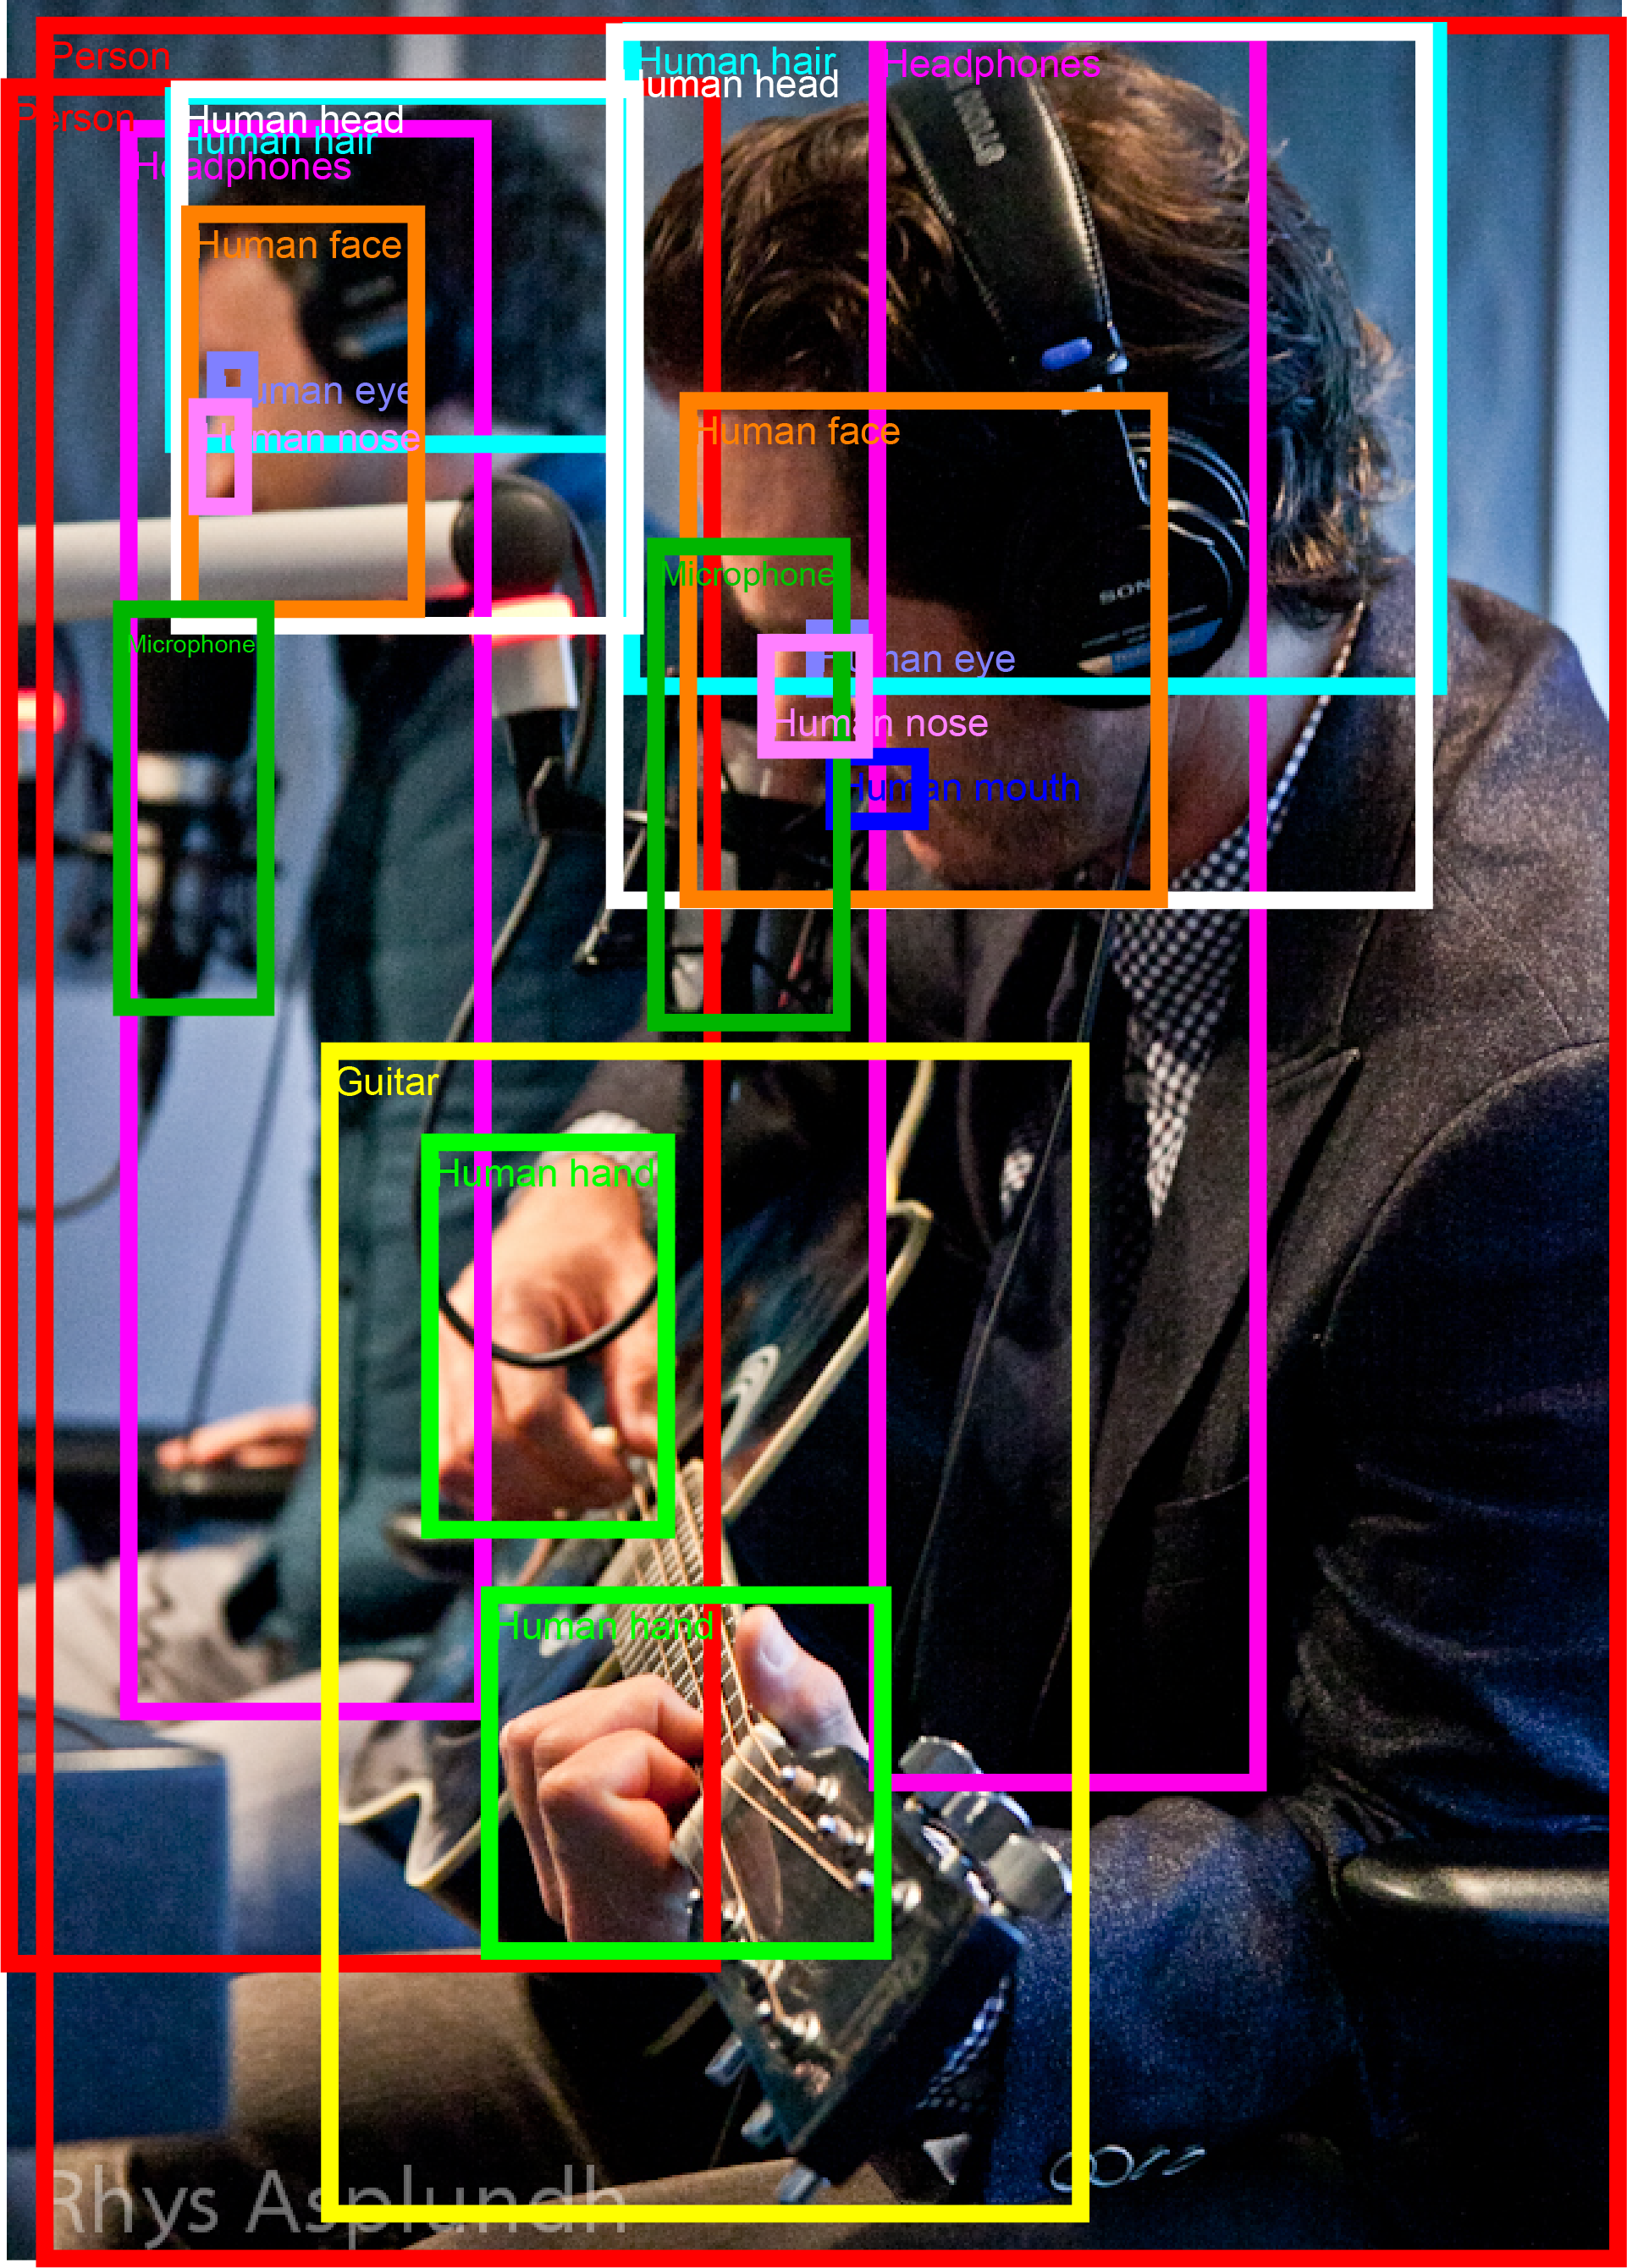
\includegraphics[width=.7\textwidth]{intro-1.png}
	\caption{\scriptsize Mark Paul Gosselaar plays the guitar by Rhys A. \cite{google:1}}
\end{figure}

The Kaggle challenge created by Google called Open Images 2019 - Object Detection \cite{kaggle} motivates this project. This Kaggle was created using the recent data set announced, the Open Images Dataset v5 \cite{google:1}. This project proposes to show some strategies to solve the problem, given a deep dive into some deep neural network architectures. 

\subsection{Problem Statement}

As described, the problem is going to be divided into two, the problem to create the correct bounding box and the problem to classify it. The idea is to create a simple pipeline with two models concatenated, and each model is going to optimize each technique.

The first model, called Bounding Box Identifier, is responsible for identifying all objects that could be classified by the Image Classifier Model. The loss function of this model is going to be the IoU (Intersection over Union) - described better in the next subsection.

On the other side, for the Image Classifier model, it is going to use the Categorial Crossentropy as a loss function.

\begin{figure}[ht]
	\centering
	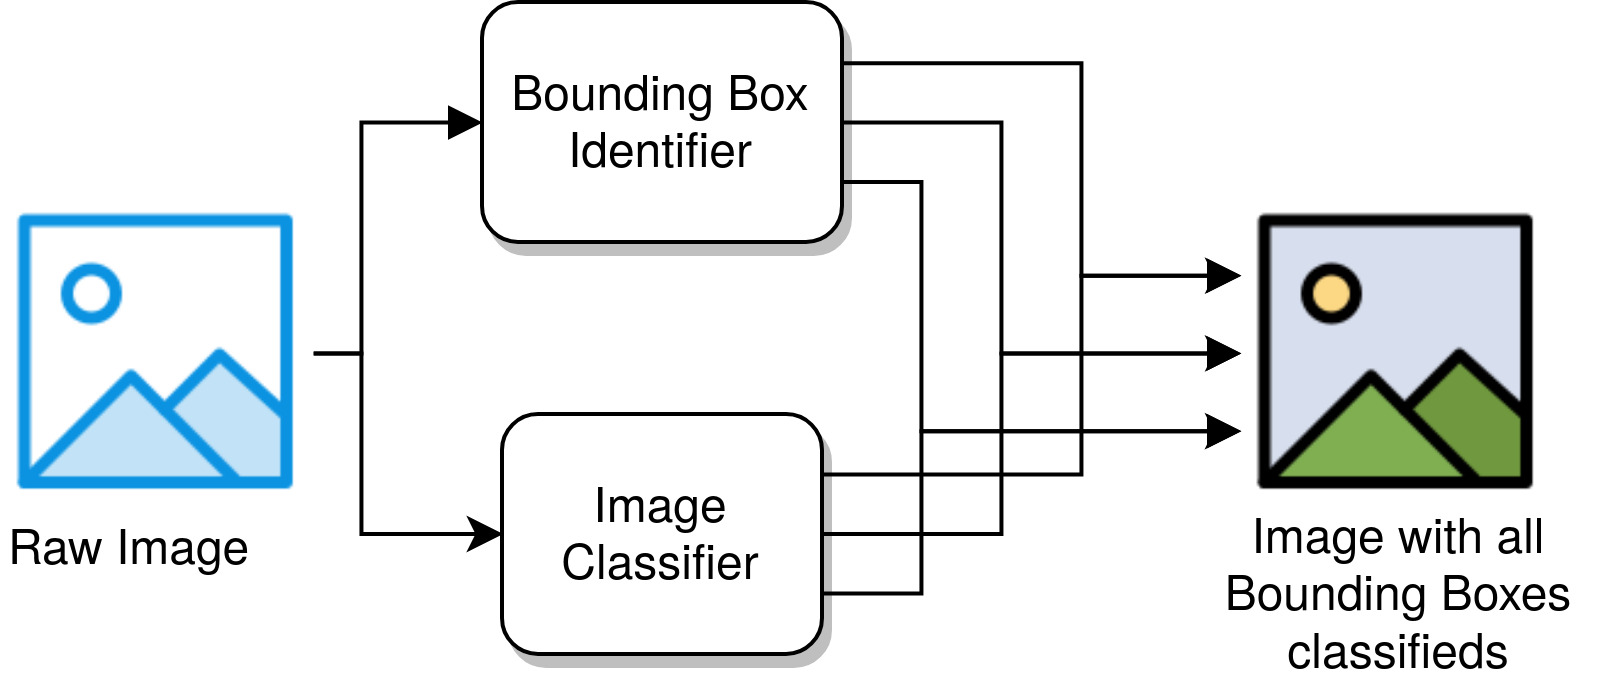
\includegraphics[width=1\textwidth]{high-level-architecture.jpg}
	\caption{\scriptsize High level Model Pipeline}
\end{figure}

It is import to explaining more about the loss functions. 

The Categorical Crossentropy used in the Classifier model is straightforward since it is a multiclass classifier. The idea is to compare for each class each distribution of the predictions made with the labeled distribution.

The IoU metric used as loss function arrives because mAP derives directly from the IoU. Since the mAP is going to be used as a metric to compare all models, it sounds reasonable to use IoU as a loss function to be optimized in the model responsible for creating the Bounding Boxes.

In the first step, the project starts to using the Transfer Learning technique in many famous networks - such as ResNet-N layers \cite{resnet}, Inception-V4 \cite{inception}, Xception \cite{xception}, and Inception-ResNets \cite{inception} - for both models, Object Identification, and Classifier. With Transfer Learning, we expect to achieve some reasonable results.

For the second and final step of the project, this work proposes to create, at minimum, one new architecture that could face other architectures seen above.

\subsection{Metrics}

The metric proposed by Google in the competition is the mean Average Precision (mAP) \cite{map}, a very didactic explanation about the metric could be found in here \cite{medium:1} and \cite{medium:2}.

The mAP metric could be defined as

{\centering
	\begin{equation*}
	mAP = \frac{\sum\limits_{c=1}^{C}AP_c} {C}
	\end{equation*}}

where $C$ value is the number of all categories (classes).

To understand $AP_c$, it must comprehend first what is $IoU$. $IoU$ is the Intersection over Union, and it is equal to the ratio of the area of intersection and area of the union of the predicted bounding box (created by the model) and Ground-truth bounding box (previously annotated).


\begin{figure}[!ht]
	\centering
	\subfloat[\scriptsize  Difference between a predict bounding box with a Ground-truth bouding box \cite{pyimage}]{{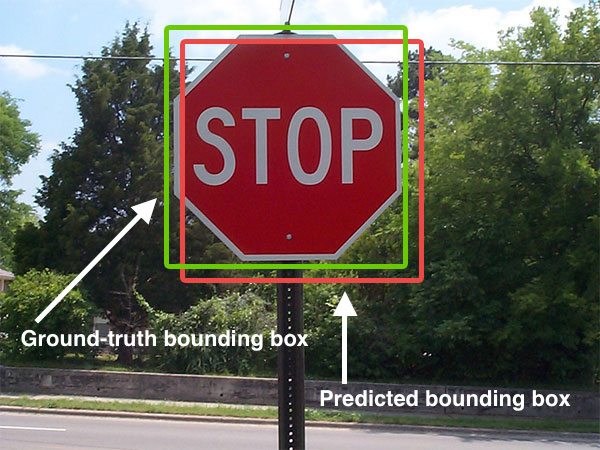
\includegraphics[width=5cm]{iou_stop_sign} }}%
	\qquad
	\subfloat[\scriptsize IoU visual represented \cite{pyimage}]{{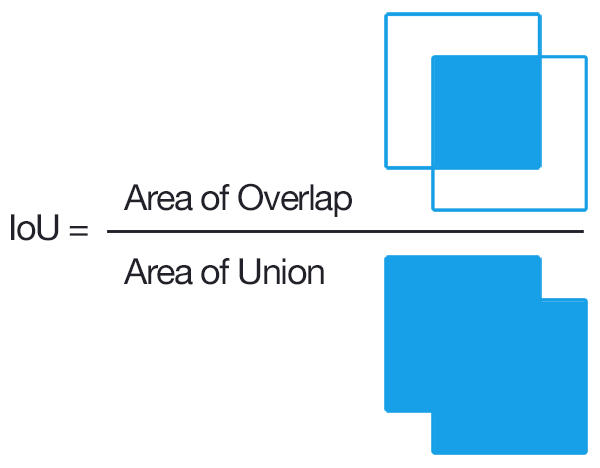
\includegraphics[width=5cm]{iou_equation} }}%
	%\caption{2 Figures side by side}%
	\label{fig:example}%
\end{figure}

Here, it is going to define:
\begin{align*}
TruePositive\ \dot=&\ IoU > 0.5 \\
FalsePositive\ \dot=&\ IoU < 0.5 \\
&or\ Duplicated PredictBoundingBox \\
FalseNegative\ \dot=&\ IoU > 0.5\ \\ 
&and \ WrongClassification
\end{align*}

With the concept of True Positive (TP), True Negatives (TN), and False Positives (FN) defined, it is possible to create a Precision-Recall Curve, which defines a function that gives a precision based on the recall.

\begin{figure}[!ht]
	
	\centering
	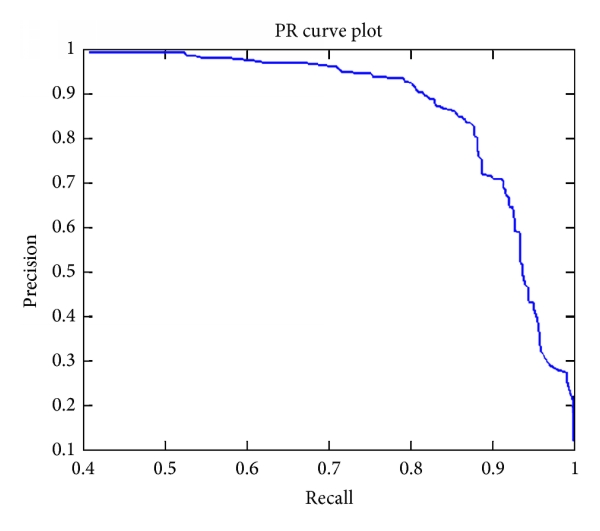
\includegraphics[width=.5\textwidth]{precision-recall.png}
	\caption{\scriptsize Precision-Recall curve \cite{medium:1}}
	
\end{figure}

So by definition, $AP_c$ (Average Precision of some category c), is defined as an Area Under the Curve ($AUC$) of the Precision-Recall curve.

{\centering
	\begin{equation*}
	AP_c = \int_{0}^{1} p(r) dr
	\end{equation*}
	where $p(r)$ is the precision defined in function of recall.}

It is essential to retain that in this project it is going to be used $AP_{50}$ (which uses a threshold of 0.5 in $IoU$ to define $TP$), but other average precisions metrics could be used, like, $AP_{75}$ (with $IoU$ threshold of 0.75) or $AP_{90}$ (with $IoU$ threshold of 0.90).

\section{Analysis}
\subsection{Data Exploration}
\subsection{Exploratory Visualization}
\subsection{Algorithms and Techniques}
\subsection{Benchmark}
\section{Methodology}
\subsection{Data Preprocessing}
\subsection{Implementation}
\subsection{Refinement}
\section{Results}
\subsection{Model Evaluation and Validation}
\subsection{Justification}
\section{Conclusion}
\subsection{Free-Form Visualization}
\subsection{Reflection}
\subsection{Improvement}

\bibliographystyle{unsrt}
\bibliography{references.bib}{}
\end{document}